\documentclass[12pt,twoside]{report}
\usepackage[a4paper,width=180mm,top=25mm,bottom=25mm,bindingoffset=6mm]{geometry}
\usepackage[utf8]{inputenc}
\usepackage[vietnamese,english]{babel}
\usepackage{placeins}
\usepackage{listings}  
\usepackage{graphicx}
\usepackage{multirow}
\graphicspath{{images/}{../images/}}

\title{
    {Thiết kế và triển khai hệ thống phát hiện xâm nhập dựa trên kĩ thuật máy học}\\
    {
\includegraphics[width=4cm]{logo}}
}
\author{
    Nguyễn Đức Thông
    \\
    Phạm Ngọc Hiếu Minh
    \\
    Trần Thanh Tín
}

\begin{document}
\selectlanguage{vietnamese}
\pagenumbering{gobble}
\maketitle
\newpage
\tableofcontents
\listoffigures
\listoftables
\newpage

    \pagenumbering{arabic}
    \chapter{Giới thiệu}
    \subsection{Đề tài}
\subsection{Đặt vấn đề}
\subsection{Mục tiêu}
    \newpage
    \chapter{Lí thuyết}
    \section{Hệ thống phát hiện xâm nhập}
    \subsection{Giới thiệu}
IDS ( Intrusion Detection System – hệ thống phát hiện xâm nhập) là một hệ thống giám sát lưu lượng mạng, có khả năng phát hiện các hoạt động khả nghi và cảnh báo cho hệ thống hoặc người quản trị mạng.
IDS phát hiện dựa trên các dấu hiệu đặc biệt về các nguy cơ đã biết hoặc dựa trên việc so sánh lưu lượng mạng hiện tại với baseline.
Trong đó baseline cho những hành vi bình thường được thiết lập bởi hồ sơ người dùng, máy chủ, hoặc hoạt động mạng trong quá trình học.
Sau khi quá trình học kết thúc, những phát hiện bất thường được tìm ra sau quá trình thăm dò của IDS bị chệch đi so với baseline này.
Phát hiện xâm nhập là một công việc khó khăn do sự phát triển nhanh chóng các của mạng lưới mạng, quá nhiều môi trường máy tính dẫn đến tính bất đồng bộ, nhiều giao thức mạng và sự phân loại đáng kể của các ứng dụng thông dụng và độc quyền. 
Hầu hết IDS sử dụng các dấu hiệu đặc biệt về nguy cơ xâm nhập đã biết( tương tự đối với cách mà các chương trình diệt virus hiện nay sử dụng để phát hiện và diệt virus), và sự khác biệt ứng xử của dấu hiệu xâm nhập so với những dấu hiệu đến từ người dùng thông thường.
\par
IDS thường được đặt ở nhiều vị trí trong hệ thống mạng, trong đó, vị trí phía sau Firewall được nhiều nhà quản trị tin dùng nhất. ở vị trí này, IDS có nhiệm vụ phân tích các gói tin đã được Firewall thông qua, xác định các dấu hiệu đã được định nghĩa mà Firewall không thể kiểm tra hoặc ngăn chặn. Từ các dấu hiệu này, IDS cung cấp thông tin và đưa ra các cảnh báo cho người quản trị viên.
\par
Với việc bảo vệ an toàn thông tin mạng ở một mức độ cao. 
Nhiều chuyên gia cho rằng IDS có giá trị giống như Firewall và VPN là ngăn ngừa các cuộc tấn công mà trong đó IDS cung cấp sự an toàn bằng cách trang bị cho bạn thông tin về các cuộc tấn công.
Chính vì điều này, IDS có thể đáp ứng nhu cầu về an toàn hệ thống bằng cách cảnh báo về khả năng có thể xảy ra của các cuộc tấn công và đôi khi bên cạnh các cảnh báo đúng thì chúng cũng mắc phải một số nhầm lẫn dần đến các cảnh báo chưa chính xác.
\subsection{Chức năng}
Nhìn chung, bản thân IDS không có khả năng tự động ngăn chặn các cuộc tấn công, tuy nhiên, các phiên bản hiện đại của IDS như IPS (sẽ được nhắc đến ở những chương sau) đã có thể thực hiện nhiều vai trò hơn và có thể ngăn chặn các cuộc tấn công khi nó xảy ra. 
Thực tế, IDS dường như chỉ thông báo cho chúng ta biết rằng mạng đang có dấu hiệu bị tấn công và đang ở trong giai đoạn nguy hiểm.
\par
Hệ thống phát hiện xâm nhập cho phép các tổ chức bảo vệ hệ thống mạng khỏi những đe dọa với việc gia tăng kết nối mạng và sự tin cậy của hệ thống thông tin, bổ sung cho những điểm yếu của hệ thống khác…
Sau đây là một vài lý do mà một hệ thống nên sử dụng IDS:
\begin{itemize}
\item Bảo vệ tính toàn vẹn dữ liệu, đảm bảo sự nhất quán của dữ liệu trong hệ thống. Các biện pháp đưa ra có khả năng ngăn chặn được sử thay đổi bất hợp pháp hoặc phá hoại dữ liệu.
\item Bảo vệ tính riêng tư, nghĩa là đảm bảo cho người sử dụng khai thác tài nguyên của hệ thống theo đúng chức năng nhiệm vụ đã được phân quyền, ngăn chặn được sự truy cập thong tin bất hợp pháp.
\item Bảo vệ tính bí mật, giữ cho thông tin không bị để lộ ra ngoài phạm vi cho phép.
\item Bảo vệ tính khả dụng, nghĩa là hệ thống luôn sẵn sàng thực hiện yêu cầu truy cập thông tin của người dùng hợp pháp.
\item Cung cấp thông tin về sự truy cập, đưa ra các chính sách đối phó, khôi phục, sửa chữa…
\end{itemize}
Về cơ bản, hệ thống IDS có thể giúp chúng ta ngăn ngừa các sự kiện tấn công trước khi nó xảy ra, cung cấp một số các giải pháp cho mạng và máy chủ, thậm chí cũng có thể hoạt động như một chuông báo động. 
Tuy nhiên chức năng chính của nó là thông báo cho người quản trị biết về các sự kiện có liên quan đến an ninh hệ thống đang sắp sửa xảy ra trong mạng và hệ thống mà người quản trị hiện đang kiểm soát.
\par
Thông thường, để phân loại IDS (IPS), người ta thường dựa vào đặc điểm của nguồn dữ liệu thu thập được. Trong trường hợp này, các hệ thống IDS được chia thành hai loại phổ biến như sau:
\begin{itemize}    
\item Host-Based IDS (HIDS): Sử dụng dữ liệu kiểm tra từ một máy trạm đơn để phát hiện xâm nhập.
\item Network-Based IDS (NIDS): Sử dụng dữ liệu trên toàn bộ lưu thông mạng, cùng với dữ liệu kiểm tra từ một hoặc một vài máy trạm để phát hiện xâm nhập.
\end{itemize}
\subsection{NIDS}
Hệ thống IDS dựa trên mạng sử dụng bộ dò và bộ cảm biến được cài đặt trên toàn mạng. Những bộ dò này theo dõi trên mạng với mục đích tìm kiếm những lưu lượng mạng khớp với những dấu hiệu được mô tả, định nghĩa từ trước. Những bộ cảm biến thu nhận và phân tích lưu lượng trong hệ thống thời gian thực. Khi nhận được mẫu lưu lượng hay dấu hiệu, bộ cảm biến gửi cảnh báo đến trạm quản trị và có thể được cấu hình nhằm tìm ra biện pháp ngăn chặn những xâm nhập xa hơn. NIDS là tập hợp nhiều cảm biến được cài đặt ở trên toàn mạng nhằm theo dõi những gói tin trong mạng, so sánh với mạng được định nghĩa để phát hiện đó là tấn công hay không.
\par
NIDS được đặt giữa hệ thống mạng bên trong và hệ thống mạng bên ngoài để giám sát toàn bộ lưu lượng vào ra. Có thể là một thiết bị phần cứng riêng biệt được thiết lập sẵn hay phần mềm cài đặt trên máy tinh, chủ yếu dùng để đo lưu lượng mạng được sử dụng.
\begin{figure}[!htbp]
    \centering
    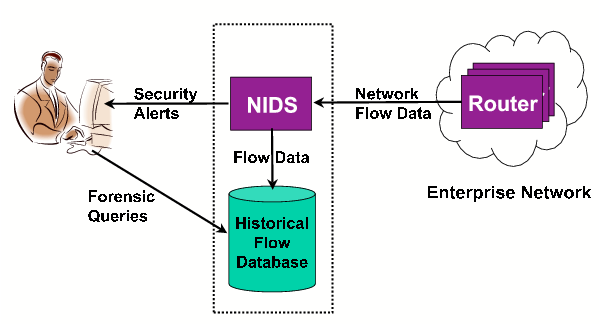
\includegraphics[scale=0.7]{nids}
    \caption{Luồng hoạt động của NIDS}
    \label{fig:x cubed graph}
\end{figure}
\FloatBarrier
NIDS giám sát toàn bộ mạng con của nó bằng cách lắng nghe tất cả các luồng dữ liệu trên mạng con đó. (Nó thay đổi chế độ hoạt động của card mạng NIC vào trong chế độ promisuous). Bình thường, một NIC hoạt động ở chế độ nonpromisuous nghĩa là nó chỉ nhận các gói tin mà có địa chỉ MAC khớp với địa chỉ của nó, các gói tin khác sẽ không nhận, hoặc không xử lý và bị loại bỏ.
Để giám sát tất cả các đường truyền trong mạng con, NIDS phải chấp nhận tất cả các gói tin và chuyển chúng tới ngăn xếp để xử lý. Do vậy nó sẽ phải cài đặt chế độ hoạt động cho card mạng là promisuous.
\newline
\newline
\textbf{Ưu điểm}
\begin{itemize}
    \item Chi phí triển khai thấp
    \item Phát hiện được các cuộc tấn công mà HIDS bỏ qua. 
    \newline Khác với HIDS, NIDS kiểm tra header của tất cả các gói tin vì thế hầu như không bỏ sót các dấu hiệu xuất phát từ đây.
    \item Khó xóa bỏ dấu vết (evidence)
    \item Phát hiện và đối phó kịp thời
    \item Có tính độc lập cao
\end{itemize}
\textbf{Nhược điểm}
\begin{itemize}
    \item Bị hạn chế với Switch
    \item Hạn chế về hiệu năng
    \item Tăng băng thông mạng
    \item Một hệ thống NIDS thường gặp khó khăn trong việc xử lý các cuộc tấn công trong một phiên được mã hóa
    \item Một hệ thống NIDS cũng gặp khó khăn khi phát hiện các cuộc tấn công mạng từ các gói tin phân mảnh
\end{itemize}
\subsection{HIDS}
Host-based IDS tìm kiếm dấu hiệu của xâm nhập trong một máy chủ cục bộ; thường sử dụng các cơ chế kiểm tra và phân tích các thông tin được lưu lại. 
Chủ yếu tìm kiếm các hoạt động bất thường như đăng nhập, truy cập tập tin không được cấp phép, bước leo thang các đặc quyền không được chấp nhận. 
Kiến trúc IDS này thường dựa trên các luật (rule-based) để phân tích các hoạt động. 
Ví dụ, đặc quyền của người sử dụng ở quyền bậc cao chỉ có thể thành công thông qua lệnh su-select user, như vậy những hành vi đăng nhập liên tục vào tài khoản root có thể được coi là một cuộc tấn công.
\newline
\newline
\textbf{Ưu điểm}
\begin{itemize}
    \item Xác định được kết quả của cuộc tấn công
    \item Khả năng giám sát các hoạt động cụ thể của hệ thống
    \item Phát hiện các hoạt động xâm nhập mà NIDS không phát hiện được: chẳng hạn kẻ tấn công sử dụng bàn phím xâm nhập vào một máy chủ sẽ không bị NIDS phát hiện.
    \item Không yêu cầu thêm phần cứng
\end{itemize}
\textbf{Nhược điểm}
\begin{itemize}
    \item Khó quản trị
    \item Nguồn thông tin phân tích không an toàn
    \item Hệ thống host-based khá đắt
    \item Chiếm tài nguyên hệ thống
\end{itemize}

    \section{Khai phá dữ liệu}
    \subsection{Khái niệm}
Là quá trình tính toán để tìm ra các mẫu trong các bộ dữ liệu lớn liên quan đến các phương pháp tại giao điểm của máy học, thống kê và các hệ thống cơ sở dữ liệu. 
Đây là một lĩnh vực liên ngành của khoa học máy tính. Mục tiêu tổng thể của quá trình khai thác dữ liệu là trích xuất thông tin từ một bộ dữ liệu và chuyển nó thành một cấu trúc dễ hiểu để sử dụng tiếp. 
Ngoài bước phân tích thô, nó còn liên quan tới cơ sở dữ liệu và các khía cạnh quản lý dữ liệu, xử lý dữ liệu trước, suy xét mô hình và suy luận thống kê, các thước đo thú vị, các cân nhắc phức tạp, xuất kết quả về các cấu trúc được phát hiện, hiện hình hóa và cập nhật trực tuyến.
\subsection{Các bước trong quá trình khai phá}
Quá trình được thực hiện qua 9 bước:
\begin{enumerate}
    \item \textbf{Tìm hiểu lĩnh vực của bài toán (ứng dụng)}: Các mục đích của bài toán,
    các tri thức cụ thể của lĩnh vực.
    \item \textbf{Tạo nên (thu thập) một tập dữ liệu phù hợp.}
    \item \textbf{Làm sạch và tiền xử lý dữ liệu.}
    \item \textbf{Giảm kích thức của dữ liệu, chuyển đổi dữ liệu}: Xác định thuộc tính quan
    trọng, giảm số chiều (số thuộc tính), biểu diễn bất biến.
    \item \textbf{Lựa chọn chức năng khai phá dữ liệu}: Phân loại, gom cụm, dự báo, sinh
    ra các luật kết hợp.
    \item \textbf{Lựa chọn/ Phát triển (các) giải thuật khai phá dữ liệu phù hợp.}
    \item \textbf{Tiến hành khai phá dữ liệu.}
    \item \textbf{Đánh giá mẫu thu được và biểu diễn tri thức}: Hiển thị hóa, chuyển đổi, bỏ
    đi các mẫu dư thừa,…
    \item \textbf{Sử dụng tri thức được khai phá.}
\end{enumerate}
Quá trình khám phá tri thức theo cách nhìn của giới nghiên cứu về các hệ
thống dữ liệu và kho dữ liệu về quá trình khám phá tri thức
\begin{itemize}
    \item Chuẩn bị dữ liệu \textit{(data preparation)}, bao gồm các quá trình làm sạch dữ liệu
    \textit{(data cleaning)}, tích hợp dữ liệu \textit{(data integration)}, chọn dữ liệu \textit{(data selection)},
    biến đổi dữ liệu \textit{(data transformation)}.
    \item Khai thác dữ liệu \textit{(data mining)}: xác định nhiệm vụ khai thác dữ liệu và lựa
    chọn kỹ thuật khai thác dữ liệu. Kết quả cho ta một nguồn tri thức thô.
    \item Đánh giá \textit{(evaluation)}: dựa trên một số tiêu chí tiến hành kiểm tra và lọc
    nguồn tri thức thu được. 
    \item Triển khai \textit{(deployment)}.
    \item Quá trình khai thác tri thức không chỉ là một quá trình tuần tự từ bước đầu
    tiên đến bước cuối cùng mà là một quá trình lặp và có quay trở lại các bước đã qua.
\end{itemize}
\begin{figure}[!htbp]
    \centering
    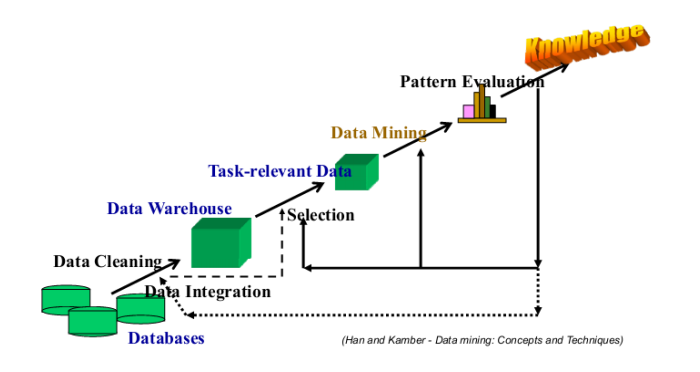
\includegraphics[scale=0.7]{data_mining}
    \caption{Quá trình khai phá tri thức}
    \label{fig:x cubed graph}
\end{figure}
\FloatBarrier
\subsection{Ứng dụng của khai phá dữ liệu}
\begin{itemize}
    \item Kinh tế - ứng dụng trong kinh doanh, tài chính, tiếp thị bán hàng, bảo hiểm,
    thương mại, ngân hàng, … Đưa ra các bản báo cáo giàu thông tin; phân tích rủi ro
    trước khi đưa ra các chiến lược kinh doanh, sản xuất; phân loại khách hàng từ đó phân định thị trường, thị phần; …
    \item Khoa học: Thiên văn học – dự đoán đường đi các thiên thể, hành tinh, …;
    Công nghệ sinh học – tìm ra các gen mới, cây con giống mới, …; …
    \item Web: các công cụ tìm kiếm.  
\end{itemize}
    \section{Máy học}
    \subsection{Giới thiệu}
Những năm gần đây, AI - Artificial Intelligence (Trí Tuệ Nhân Tạo), và cụ thể hơn là Machine Learning (Học Máy hoặc Máy Học) nổi lên như một bằng chứng của cuộc cách mạng công nghiệp lần thứ tư (1 - động cơ hơi nước, 2 - năng lượng điện, 3 - công nghệ thông tin). 
Trí Tuệ Nhân Tạo đang len lỏi vào mọi lĩnh vực trong đời sống mà có thể chúng ta không nhận ra. 
Xe tự hành của Google và Tesla, hệ thống tự tag khuôn mặt trong ảnh của Facebook, trợ lý ảo Siri của Apple, hệ thống gợi ý sản phẩm của Amazon, hệ thống gợi ý phim của Netflix, máy chơi cờ vây AlphaGo của Google DeepMind, …, chỉ là một vài trong vô vàn những ứng dụng của AI/Machine Learning.
\par
Machine Learning là một tập con của AI. 
Theo định nghĩa của Wikipedia, Machine learning is the subfield of computer science that “gives computers the ability to learn without being explicitly programmed”. 
Nói đơn giản, Machine Learning là một lĩnh vực nhỏ của Khoa Học Máy Tính, nó có khả năng tự học hỏi dựa trên dữ liệu đưa vào mà không cần phải được lập trình cụ thể.
\par
Những năm gần đây, khi mà khả năng tính toán của các máy tính được nâng lên một tầm cao mới và lượng dữ liệu khổng lồ được thu thập bởi các hãng công nghệ lớn, Machine Learning đã tiến thêm một bước dài và một lĩnh vực mới được ra đời gọi là Deep Learning (Học Sâu - thực sự tôi không muốn dịch từ này ra tiếng Việt). 
Deep Learning đã giúp máy tính thực thi những việc tưởng chừng như không thể vào 10 năm trước: phân loại cả ngàn vật thể khác nhau trong các bức ảnh, tự tạo chú thích cho ảnh, bắt chước giọng nói và chữ viết của con người, giao tiếp với con người, hay thậm chí cả sáng tác văn hay âm nhạc
\subsection{Phân nhóm các thuật toán}
Theo phương thức học, các thuật toán Machine Learning thường được chia làm 4 nhóm:
\begin{itemize}
\item Supervise learning (học có giám sát)
\item Unsupervised learning ( học không có giám sát)
\item Semi-supervised lerning ( Học bán giám sát)
\item Reinforcement learning ( Học củng cố)
\end{itemize}
\begin{enumerate}
\item \textbf{Học có giám sát (Supervised Learning)}
\par
Supervised learning là thuật toán dự đoán đầu ra (outcome) của một dữ liệu mới (new input) dựa trên các cặp (input, outcome) đã biết từ trước. 
Cặp dữ liệu này còn được gọi là (data, label), tức (dữ liệu, nhãn). 
Supervised learning là nhóm phổ biến nhất trong các thuật toán Machine Learning
\begin{enumerate}
\item \textbf{Classification (Phân loại)}: Một bài toán được gọi là classification nếu các label của input data được chia thành một số hữu hạn nhóm. 
Ví dụ: Gmail xác định xem một email có phải là spam hay không; các hãng tín dụng xác định xem một khách hàng có khả năng thanh toán nợ hay không. 
Ba ví dụ phía trên được chia vào loại này
\par
\item \textbf{Regression (Hồi quy)}
Nếu label không được chia thành các nhóm mà là một giá trị thực cụ thể. Ví dụ: một căn nhà rộng x m2x m2, có yy phòng ngủ và cách trung tâm thành phố z kmz km sẽ có giá là bao nhiêu?
\par
Gần đây Microsoft có một ứng dụng dự đoán giới tính và tuổi dựa trên khuôn mặt. 
Phần dự đoán giới tính có thể coi là thuật toán Classification, phần dự đoán tuổi có thể coi là thuật toán Regression. 
Chú ý rằng phần dự đoán tuổi cũng có thể coi là Classification nếu ta coi tuổi là một số nguyên dương không lớn hơn 150, chúng ta sẽ có 150 class (lớp) khác nhau
\end{enumerate}
\item \textbf{Học không giám sát ( Unsupervise learning)}
\par
Trong thuật toán này, chúng ta không biết được outcome hay nhãn mà chỉ có dữ liệu đầu vào. 
Thuật toán unsupervised learning sẽ dựa vào cấu trúc của dữ liệu để thực hiện một công việc nào đó, ví dụ như phân nhóm (clustering) hoặc giảm số chiều của dữ liệu (dimension reduction) để thuận tiện trong việc lưu trữ và tính toán.
\par
Một cách toán học, Unsupervised learning là khi chúng ta chỉ có dữ liệu vào XX mà không biết nhãn YY tương ứng.
Những thuật toán loại này được gọi là Unsupervised learning vì không giống như Supervised learning, chúng ta không biết câu trả lời chính xác cho mỗi dữ liệu đầu vào. 
Giống như khi ta học, không có thầy cô giáo nào chỉ cho ta biết đó là chữ A hay chữ B. 
Cụm không giám sát được đặt tên theo nghĩa này.
\par
Các bài toán Unsupervised learning được tiếp tục chia nhỏ thành hai loại:
\begin{enumerate}
\item \textbf{Clustering (phân nhóm)}
\par
Một bài toán phân nhóm toàn bộ dữ liệu XX thành các nhóm nhỏ dựa trên sự liên quan giữa các dữ liệu trong mỗi nhóm. 
Ví dụ: phân nhóm khách hàng dựa trên hành vi mua hàng. Điều này cũng giống như việc ta đưa cho một đứa trẻ rất nhiều mảnh ghép với các hình thù và màu sắc khác nhau, ví dụ tam giác, vuông, tròn với màu xanh và đỏ, sau đó yêu cầu trẻ phân chúng thành từng nhóm. 
Mặc dù không cho trẻ biết mảnh nào tương ứng với hình nào hoặc màu nào, nhiều khả năng chúng vẫn có thể phân loại các mảnh ghép theo màu hoặc hình dạng.
\newline
\newline
\item \textbf{Association (kết hợp)}
\par
Là bài toán khi chúng ta muốn khám phá ra một quy luật dựa trên nhiều dữ liệu cho trước. 
Ví dụ: những khách hàng nam mua quần áo thường có xu hướng mua thêm đồng hồ hoặc thắt lưng; những khán giả xem phim Spider Man thường có xu hướng xem thêm phim Bat Man, dựa vào đó tạo ra một hệ thống gợi ý khách hàng (Recommendation System), thúc đẩy nhu cầu mua sắm.
\end{enumerate}
\item \textbf{Học bán giám sát ( Semi-Supervise Learning)}
\par
Các bài toán khi chúng ta có một lượng lớn dữ liệu XX nhưng chỉ một phần trong chúng được gán nhãn được gọi là Semi-Supervised Learning. Những bài toán thuộc nhóm này nằm giữa hai nhóm được nêu bên trên.
\par
Một ví dụ điển hình của nhóm này là chỉ có một phần ảnh hoặc văn bản được gán nhãn (ví dụ bức ảnh về người, động vật hoặc các văn bản khoa học, chính trị) và phần lớn các bức ảnh/văn bản khác chưa được gán nhãn được thu thập từ internet. 
Thực tế cho thấy rất nhiều các bài toán Machine Learning thuộc vào nhóm này vì việc thu thập dữ liệu có nhãn tốn rất nhiều thời gian và có chi phí cao. 
Rất nhiều loại dữ liệu thậm chí cần phải có chuyên gia mới gán nhãn được (ảnh y học chẳng hạn). 
Ngược lại, dữ liệu chưa có nhãn có thể được thu thập với chi phí thấp từ internet.
\newline
\newline   
\item \textbf{Học củng cố ( Reinforcement Learning)}
\par
Reinforcement learning là các bài toán giúp cho một hệ thống tự động xác định hành vi dựa trên hoàn cảnh để đạt được lợi ích cao nhất (maximizing the performance). Hiện tại, Reinforcement learning chủ yếu được áp dụng vào Lý Thuyết Trò Chơi (Game Theory), các thuật toán cần xác định nước đi tiếp theo để đạt được điểm số cao nhất
\begin{figure}[!htbp]
    \centering
    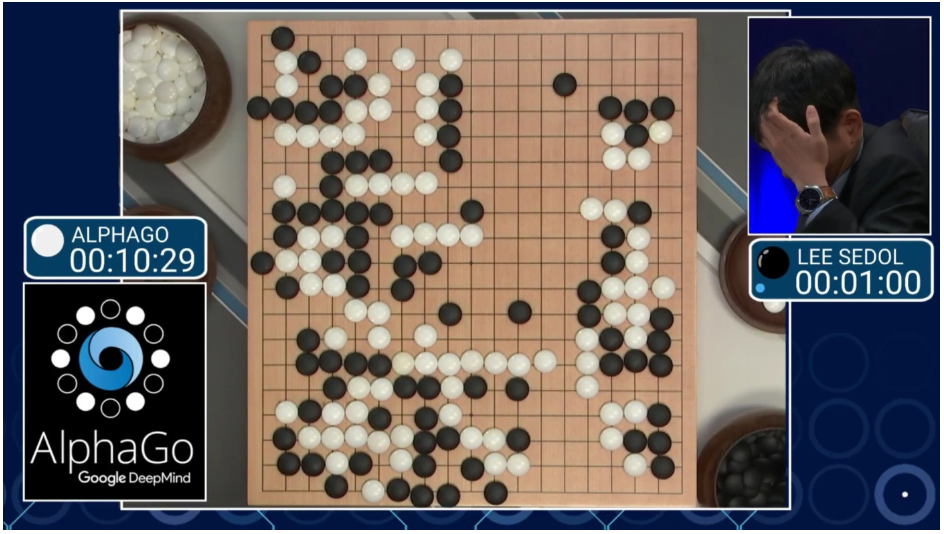
\includegraphics[scale=0.5]{reinforcement_learning}
    \caption{AlphaGo chơi cờ vây với Lee Sedol. AlphaGo là một ví dụ điển hình của Reinforcement Learing}
    \label{fig:x cubed graph}
\end{figure}
\FloatBarrier
\end{enumerate}
    \newpage
    \chapter{Công nghệ tiếp cận}
    \section{Snort 3}
    \subsubsection{Giới thiệu}
\subsubsection{Kiến trúc}
\subsubsection{Cấu hình}
\subsubsection{Mở rộng tính năng}
    \section{Scikit}
    \subsection{Giới thiệu}
\textbf{Scikit-learn} 
(viết tắt là \textbf{sklearn}) là một thư viện mã nguồn mở trong ngành machine learning, 
rất mạnh mẽ và thông dụng với cộng đồng Python, được thiết kế trên nền NumPy và SciPy. 
Scikit-learn chứa hầu hết các thuật toán machine learning hiện đại nhất, 
đi kèm với comprehensive documentations. Điểm mạnh của thư viện này là nó được sử dụng phổ biến trong academia và industry, 
do đó nó luôn được updated và có một very active user community. \break
    \section{Thuật toán KMeans}
    \subsection{Giới thiệu}
Trong thuật toán K-means clustering, chúng ta không biết nhãn (label) của từng điểm dữ liệu. 
Mục đích là làm thể nào để phân dữ liệu thành các cụm (cluster) khác nhau sao cho dữ liệu trong cùng một cụm có tính chất giống nhau.
\par
\textbf{Ví dụ}: Một công ty muốn tạo ra những chính sách ưu đãi cho những nhóm khách hàng khác nhau dựa trên sự tương tác giữa mỗi khách hàng với công ty đó (số năm là khách hàng; số tiền khách hàng đã chi trả cho công ty; độ tuổi; giới tính; thành phố; nghề nghiệp; …). 
Giả sử công ty đó có rất nhiều dữ liệu của rất nhiều khách hàng nhưng chưa có cách nào chia toàn bộ khách hàng đó thành một số nhóm/cụm khác nhau. 
Nếu một người biết Machine Learning được đặt câu hỏi này, phương pháp đầu tiên ta nghĩ đến sẽ là K-means Clustering. 
Sau khi đã phân ra được từng nhóm, nhân viên công ty đó có thể lựa chọn ra một vài khách hàng trong mỗi nhóm để quyết định xem mỗi nhóm tương ứng với nhóm khách hàng nào. 
Phần việc cuối cùng này cần sự can thiệp của con người, nhưng lượng công việc đã được rút gọn đi rất nhiều.
\par
Ý tưởng đơn giản nhất về cluster (cụm) là tập hợp các điểm ở gần nhau trong một không gian nào đó (không gian này có thể có rất nhiều chiều trong trường hợp thông tin về một điểm dữ liệu là rất lớn). 
Hình bên dưới là một ví dụ về 3 cụm dữ liệu.
\begin{figure}[!htbp]
    \centering
    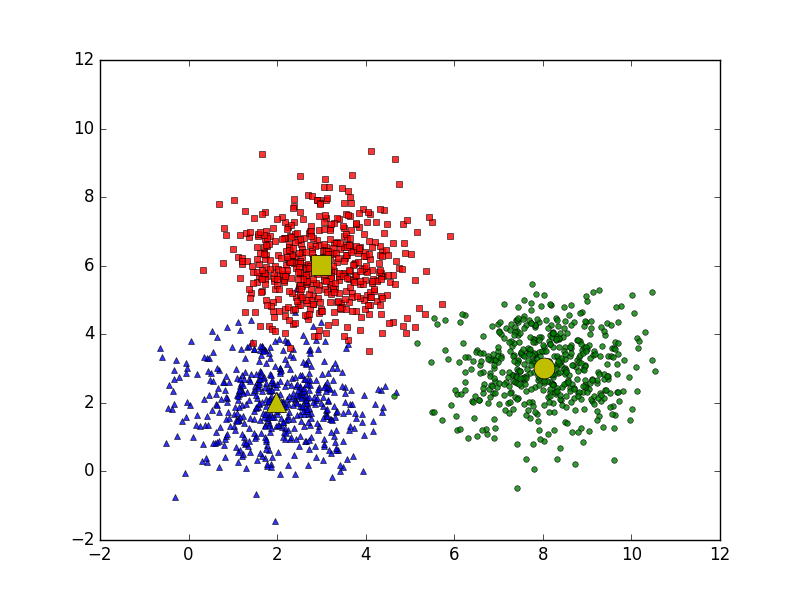
\includegraphics[scale=0.5]{kmeans}
    \caption{Bài toán với 3 clusters.}
    \label{fig:x cubed graph}
\end{figure}
\FloatBarrier
Giả sử mỗi cluster có một điểm đại diện (center) màu vàng. Và những điểm xung quanh mỗi center thuộc vào cùng nhóm với center đó. Một cách đơn giản nhất, xét một điểm bất kỳ, ta xét xem điểm đó gần với center nào nhất thì nó thuộc về cùng nhóm với center đó. Tới đây, chúng ta có một bài toán thú vị: \textit{Trên một vùng biển hình vuông lớn có ba đảo hình vuông, tam giác, và tròn màu vàng như hình trên. Một điểm trên biển được gọi là thuộc lãnh hải của một đảo nếu nó nằm gần đảo này hơn so với hai đảo kia . Hãy xác định ranh giới lãnh hải của các đảo}
\subsection{Phân tích chi tiết}
Đầu tiên là chuẩn bị dữ liệu cần phân cụm. Tiếp theo quyết định số lượng cụm (cluster) cần phân chia. Ở ví dụ này thử chọn số cluster là 3. Ở đây data được thể hiện dưới dạng các điểm cho dễ quan sát. Cự ly của các dữ liệu được hiểu là độ dài đoạn thẳng nối giữa 2 điểm với nhau.
\begin{figure}[!htbp]
    \centering
    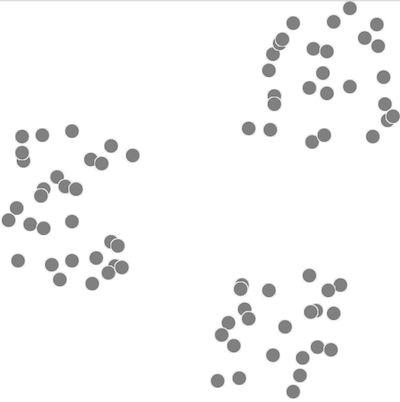
\includegraphics[scale=0.5]{kmeans_detail1}
    \caption{Cụm ban đầu.}
    \label{fig:x cubed graph}
\end{figure}
\FloatBarrier
\textbf{Bước 2}
\par
Chọn ngẫu nhiên 3 điểm làm điểm trung tâm của cluster.
\begin{figure}[!htbp]
    \centering
    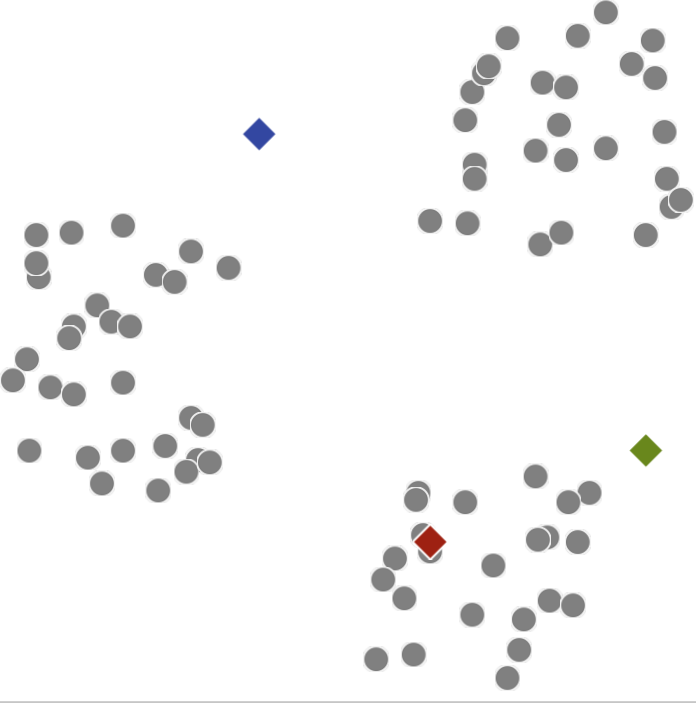
\includegraphics[scale=0.5]{kmeans_detail2}
    \caption{Chọn ngẫu nhiên trung điểm.}
    \label{fig:x cubed graph}
\end{figure}
\FloatBarrier
\textbf{Bước 3}
\par
Với các điểm dữ liệu không được chọn là điểm trung tâm thì tính toán khoảng cách từ chính điểm đó đến các cluster và quyết định cluster nào gần với mình nhất.
\begin{figure}[!htbp]
    \centering
    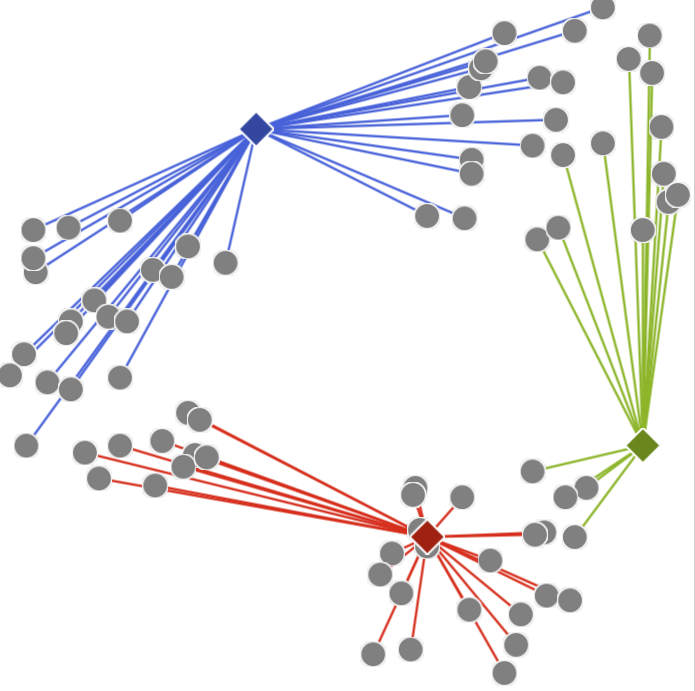
\includegraphics[scale=0.5]{kmeans_detail3}
    \caption{Tính toán khoảng cách tới điểm.}
    \label{fig:x cubed graph}
\end{figure}
\FloatBarrier
\textbf{Bước 4}
\par
Từ bước tính toán trên, tiến hành phân loại các điểm về các cluster đã quyết định(cluster gần nó nhất). Vậy là đã phân ra được 3 cụm.
\begin{figure}[!htbp]
    \centering
    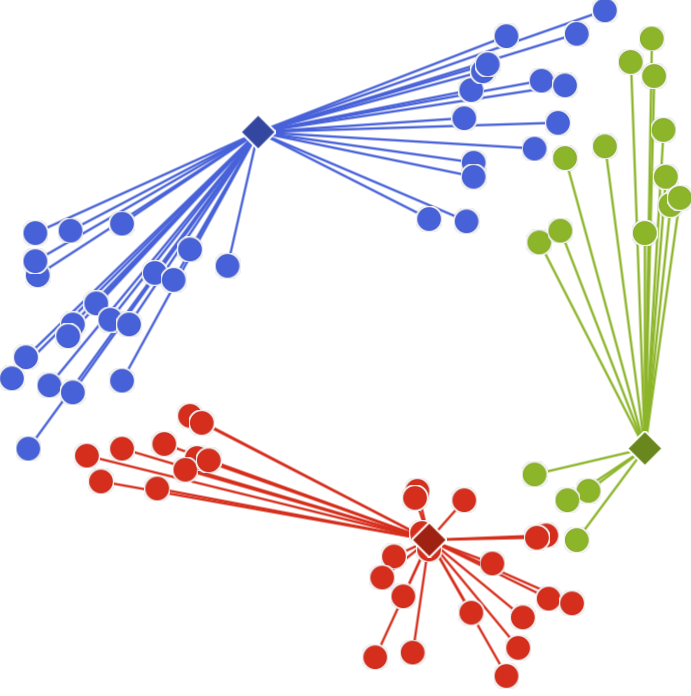
\includegraphics[scale=0.5]{kmeans_detail4}
    \caption{Phân thành 3 clusters.}
    \label{fig:x cubed graph}
\end{figure}
\FloatBarrier
\textbf{Bước 5}
\par
Bước trên chúng ta đã thu được 3 cụm, bây giờ tiến hành tính trọng tâm của các điểm dữ liệu của từng cụm. Sau đó di chuyển điểm trung tâm của cụm sang vị trí vừa tính được.
\begin{figure}[!htbp]
    \centering
    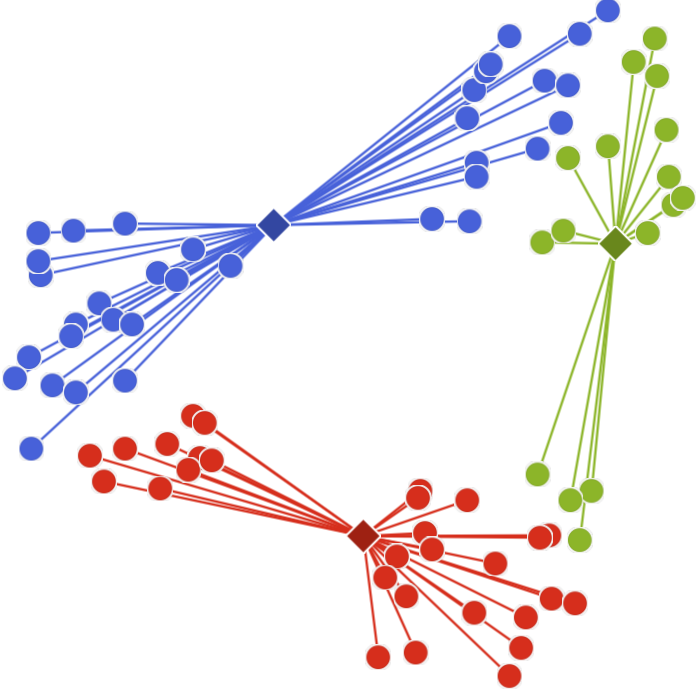
\includegraphics[scale=0.5]{kmeans_detail5}
    \caption{Tính trọng điểm.}
    \label{fig:x cubed graph}
\end{figure}
\FloatBarrier
Vị trí mà 3 điểm trung tâm của cluster vừa di chuyển đến được hiểu ngắn gọn chính là điểm trung tâm đang di chuyển đến vị trí chính xác hơn.
\newline
\textbf{Bước 6}
\par
Một lần nữa tiến hành bước 3, tính toán lại khoảng các các điểm đến các điểm trung tâm. Sau đó phân loại lại các điểm dữ liệu về các cụm.
\begin{figure}[!htbp]
    \centering
    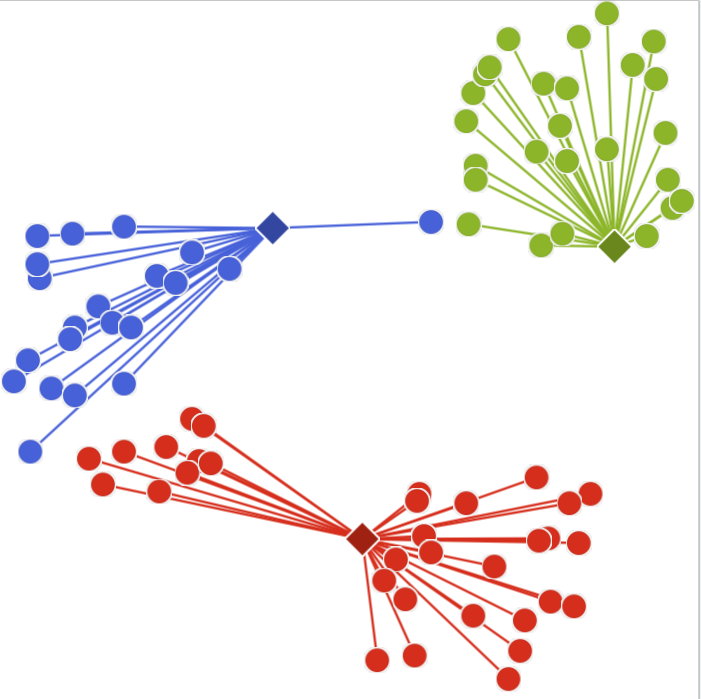
\includegraphics[scale=0.5]{kmeans_detail6}
    \caption{Tính toán lại khoảng cách.}
    \label{fig:x cubed graph}
\end{figure}
\FloatBarrier
\textbf{Bước 7}
\par
Sau đó lặp lại quá trình di chuyển cluster trung tâm và phân loại lại các điểm về các cụm gần nhất.
Quá trình này sẽ dừng khi sau khi dữ liệu sau khi phân cụm lại không thay đổi gì so với lần trước.
\begin{figure}[!htbp]
    \centering
    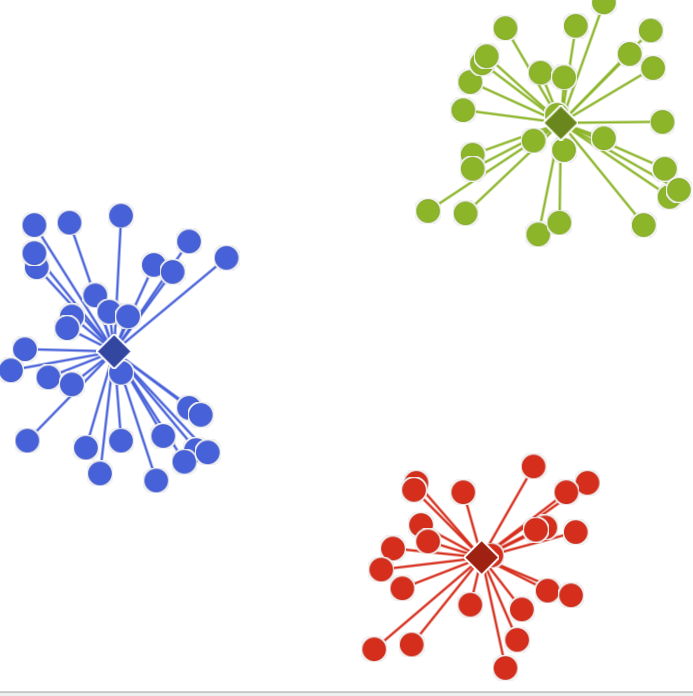
\includegraphics[scale=0.5]{kmeans_detail7}
    \caption{Kết quả.}
    \label{fig:x cubed graph}
\end{figure}
\FloatBarrier
\subsection{Lưu ý}
Trước khi sử dụng phương pháp này, chúng ta phải quyết định trước số lượng cluster, tuy nhiên trong quá trình tính toán số lượng cluster có thể khác với số lượng cluster mình dự đoán nên kết quả sẽ không chính xác.
\par
Vì vậy để giải quyết vấn đề này, để có thể chọn ra số lượng cluster thích hợp thì cần phải phân tích dữ liệu cẩn thận, chạy thử k-means với nhiều biến số số lượng cluster.
\par
Cùng ví dụ trên nếu thay số lượng cluster thành 2, kết quả phân loại sẽ thành ra như sau:
\begin{figure}[!htbp]
    \centering
    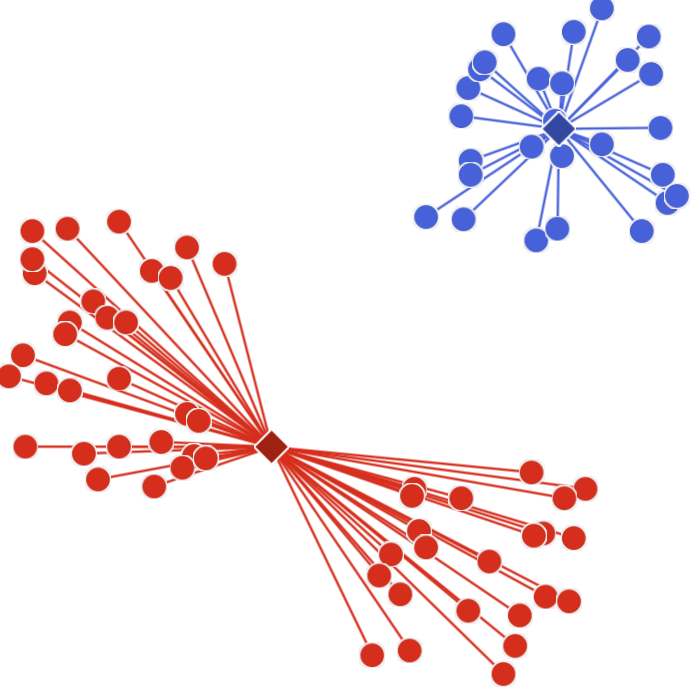
\includegraphics[scale=0.5]{kmeans_2_clusters}
    \caption{Khi chia thành 2 cụm.}
    \label{fig:x cubed graph}
\end{figure}
\FloatBarrier
    \section{Tập dữ liệu NSL-KDD}
    \subsubsection{Giới thiệu}
\subsubsection{Đặc tính}
    \section{Flatbuffer}
    FlatBuffers là một thư viện serialization đa nền tảng hiệu quả cho C++, C\#, C, Go, Java, JavaScript, TypeScript, PHP và Python. 
Ban đầu nó được tạo ra tại Google để phát triển trò chơi và các ứng dụng quan trọng khác về hiệu suất.
\subsection{Tại sao sử dụng FlatBuffers?}
\begin{itemize}
\item \textbf{Truy cập vào dữ liệu được tuần tự hóa mà không cần phân tích cú pháp / giải nén} 
- Những gì đặt ngoài FlatBuffers là nó đại diện cho dữ liệu phân cấp trong một bộ đệm nhị phân phẳng theo cách mà nó vẫn có thể được truy cập trực tiếp mà không cần phân tích cú pháp / giải nén, trong khi vẫn hỗ trợ tiến hóa cấu trúc dữ liệu (chuyển tiếp / khả năng tương thích ngược).
\item \textbf{Tốc độ và bộ nhớ hiệu quả} 
- Bộ nhớ duy nhất cần để truy cập dữ liệu của bạn là bộ đệm. Nó yêu cầu 0 phân bổ bổ sung (bằng C ++, các ngôn ngữ khác có thể thay đổi). FlatBuffers cũng rất thích hợp để sử dụng với mmap (hoặc streaming), chỉ yêu cầu một phần của bộ đệm có trong bộ nhớ. Truy cập gần với tốc độ truy cập cấu trúc thô chỉ với một thêm một hướng (một loại vtable) để cho phép phát triển định dạng và các trường tùy chọn. Đó là nhằm vào các dự án mà chi tiêu thời gian và không gian (phân bổ bộ nhớ nhiều) để có thể truy cập hoặc xây dựng dữ liệu tuần tự là không mong muốn, chẳng hạn như trong trò chơi hoặc bất kỳ ứng dụng nhạy cảm hiệu suất nào khác.
\item \textbf{Linh hoạt} 
- Các trường không bắt buọc có nghĩa là không chỉ có khả năng tương thích tốt và tương thích ngược (ngày càng quan trọng đối với các ứng dụng tồn tại lâu dài: không phải cập nhật tất cả dữ liệu với mỗi phiên bản mới!). Nó cũng có nghĩa là bạn có nhiều lựa chọn trong dữ liệu nào bạn viết và dữ liệu nào bạn không sử dụng và cách bạn thiết kế cấu trúc dữ liệu.
\item \textbf{Lượng mã nhỏ} 
- Một lượng nhỏ mã được tạo ra, rất dễ tích hợp.
\item \textbf{Kiểu dữ liệu cứng} 
- Lỗi xảy ra tại thời gian biên dịch thay vì phải viết kiểm tra thời gian chạy lặp đi lặp lại và dễ bị lỗi. Mã có thể được sinh tự động.
\item \textbf{Sử dụng thuận tiện} 
- Mã C++ được tạo cho phép truy cập và xây dựng mã. Sau đó, có chức năng tùy chọn để phân tích các lược đồ và các biểu diễn văn bản giống JSON khi chạy hiệu quả nếu cần (bộ nhớ nhanh hơn và hiệu quả hơn các trình phân tích cú pháp JSON khác).
\newline 
Mã Java và Go hỗ trợ tái sử dụng đối tượng. C\# có các trình truy cập dựa trên cấu trúc hiệu quả.
\item \textbf{Đa nền tảng và không có phụ thuộc} 
- mã C ++ sẽ hoạt động với bất kỳ gcc / clang và VS2010 gần đây nào. Đi kèm với các tệp xây dựng cho các thử nghiệm và mẫu (tệp .mk Android và cmake cho tất cả các nền tảng khác).
\end{itemize}
    \newpage
    \chapter{Triển khai và thử nghiệm}
    \section{Thiết lập dữ liệu và môi trường thử nghiệm}
\section{Kết quả và nhận xét}
    \newpage
    \chapter{Kết luận}
    \section{Nhận định}
\section{Hướng phát triển}

\newpage
\bibliography{ref}
\bibliographystyle{ieeetr}
\end{document}